\chapter{Функции.}
\section{Определение предела функции}
Рассмотрим числовую функцию $f:X\rightarrow Y$. $X, Y$ --- числовые множества.\\
\begin{example}
	\begin{enumerate}
		\item $sgn x = 
		\begin{cases}
			1, x > 0\\
			0, x = 0\\
			-1, x < 0
		\end{cases}$
		$$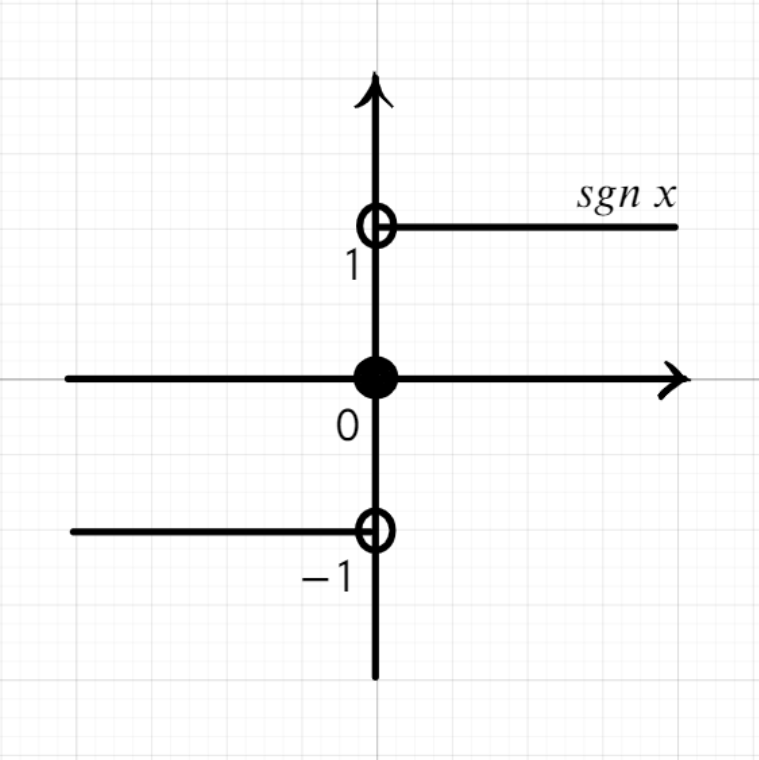
\includegraphics[scale=0.4]{images/img8.png}$$
		\item $1(x) = 
		\begin{cases}
			1, x \geqslant 0\\
			0, x < 0
		\end{cases}$ $$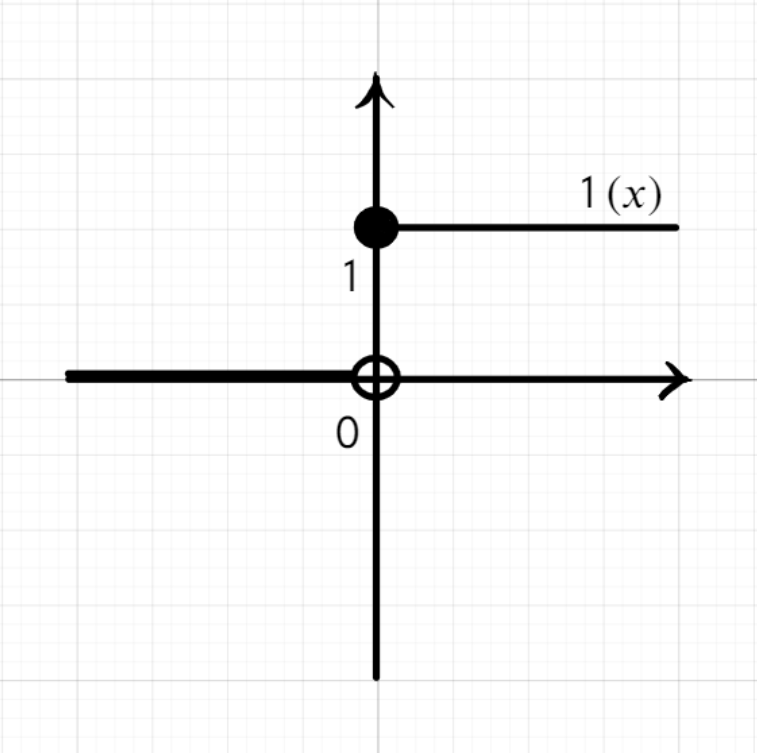
\includegraphics[scale=0.4]{images/img9.png}$$
		\item $|x| = 
		\begin{cases}
			x, x \geqslant 0\\
			-x, x < 0
		\end{cases}$ $$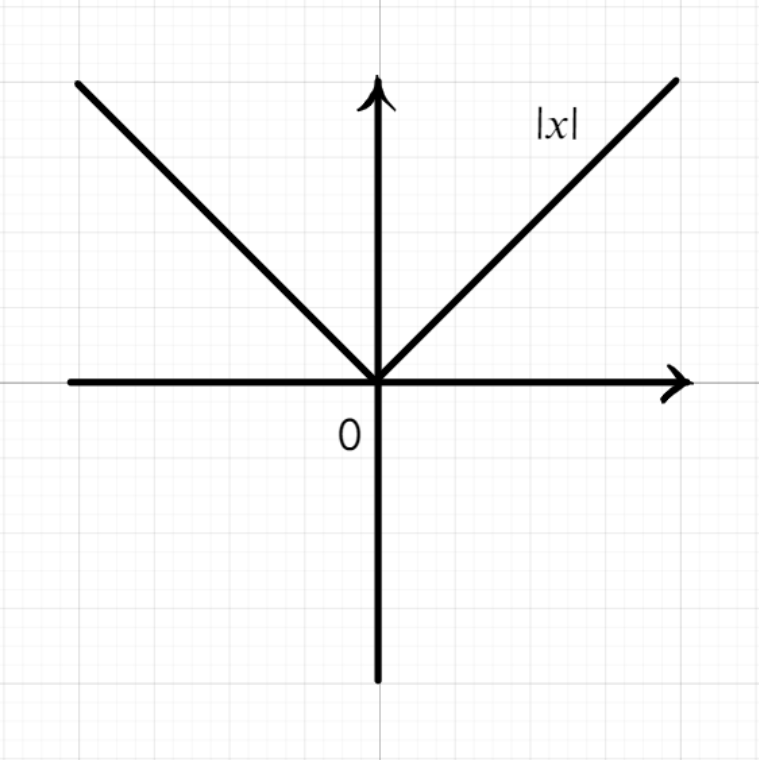
\includegraphics[scale=0.4]{images/img10.png}$$
		$|x| = x\cdot sgnx$
	\end{enumerate}
\end{example}\\\\
Предположим, что функция $f$ определена на $\dot{u}(a)$, то есть на некоторой проколотой окрестности точки $a$.\\\\
$\bullet$ \textit{Число $A\in\Rm$ называют \textbf{пределом} функции $f$ при $x\rightarrow a$, если:}
$$\forall V(A),\ \exists \dot{u}(a)\Ra f(\dot{u}(a))\subset V(A).$$\\
Иногда это определение записывают и в равносильной форме:\\\\
$\bullet$ \textit{$A$ --- \textbf{предел} $f$ при $x\rightarrow a$, если}
$$\forall V_{\varepsilon}(A),\ \exists\dot{u}_{\delta}(a),\forall x\in\dot{u}_{\delta}(a)\Ra f(a)\in V_{\varepsilon}(A).$$\\
Последнее определение можно записать и таким образом:\\\\
$\bullet$ \textit{$A$ --- \textbf{предел} $f$ при $x\rightarrow a$, если}
$$\forall\varepsilon>0,\exists\delta(\varepsilon),\forall x\in\dot{u}(a),0<|x-a|\leqslant\delta_\varepsilon\Ra|f(x)-A|\leqslant\varepsilon.$$\\
При этом употребляют, записав $\lim\limits_{x\to a}f(x) = A$, $\lim\limits_{a}f = A$, или $f(x)\underset{x\to a}{\longrightarrow}A$
\subsection{Геометрический смысл.}
$$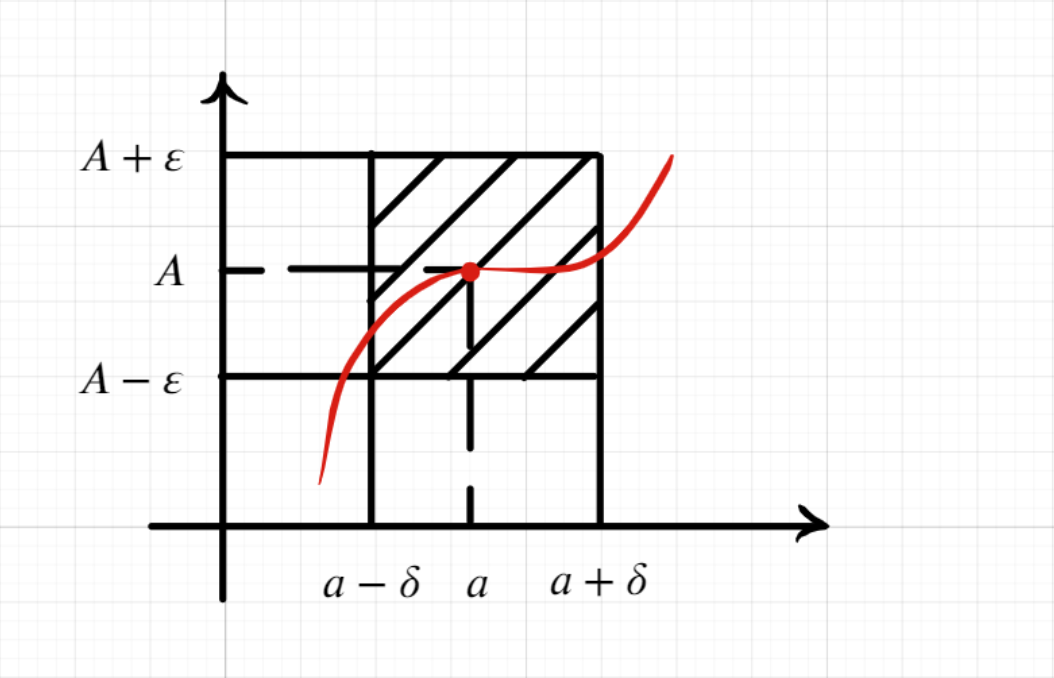
\includegraphics[scale=0.4]{images/img11.png}$$
Для любой полосы с центром в точке $A$, шириной $2\varepsilon$ (горизонтальный) $\exists$ полоса ширины $2\delta$ с центром в точке $a$ (вертикальная), что как только $x$ попадает в $\delta$-полосу, то $f(x)$ --- попадает в $\varepsilon$-полосу.
\begin{mlemma}
	Если для $$\forall\varepsilon>0,\ \exists\delta_\varepsilon>0,\ \forall x\in\dot{u}(a),\ 0<|x-a|\leqslant\delta_\varepsilon \Ra |f(x)-A|\leqslant M\cdot\varepsilon,$$ где $M$ не зависит ни от $x$, ни от $\varepsilon$, то $\lim\limits_{a}f = A$.
\end{mlemma}
\begin{Proof}
	Доказательство стандартное.
\end{Proof}
\begin{corollary}
	Из сходимости функции при $x\rightarrow a$ вытекает, что $\exists$ окрестность точки $a$, на которой функция ограничена.
\end{corollary}
\begin{Proof}
	$$\forall\varepsilon>0,\ \exists\delta_\varepsilon,\ \forall x\in D(f),\ 0<|x-a|\leqslant\delta_\varepsilon\Ra|f(x)-A|\leqslant\varepsilon$$ или $$a - \delta_\varepsilon\leqslant x\leqslant a+\delta_\varepsilon \Ra A-\varepsilon\leqslant f(x)\leqslant A+\varepsilon.$$ А это и означает ограниченность $f$ ($\varepsilon$ фиксируем).
\end{Proof}
\section{Критерий Гейне существования предела функции.}
Критерий Гейне устанавливает связь между пределом функции и пределом последовательности.
\newtheorem*{gayne}{Критерий Гейне}
\begin{gayne}
	Для того, чтобы $\lim\limits_{x\to a}f(x) = A$ необходимо и достаточно, чтобы $$\forall(x_n),\ x_n\rightarrow a,\ x_n\neq a,\ x_n\in D(f) \Ra \lim\limits_{n\to\infty}f(x_n)=A.$$
\end{gayne}
\begin{Proof}
	\textbf{Необходимость.}
	Возьмём $\forall(x_n)$, $x_n\in D(f)$, $x_n\neq a$, $x_n\rightarrow a$. Построим последовательность ($f(x_n)$). Так как $\lim\limits_{a}f = A$, то
	$$\forall\varepsilon>0, \exists\delta(\varepsilon), \forall x\in D(f), |x_n-a|\leqslant\delta_\varepsilon\Ra|f(x)-A|\leqslant\varepsilon.$$
	По построению $x_n\rightarrow a$. Поэтому для указанного $\delta_\varepsilon$ $\exists\nu_\varepsilon$ такое, что $\forall n \geqslant\nu_\varepsilon\Ra |x_n-a|\leqslant\delta_\varepsilon$. А тогда $|f(x_n)-A|\leqslant\varepsilon$.
	Таким образом,
	$$\forall\varepsilon>0, \exists\nu_\varepsilon, \forall n\geqslant\nu_\varepsilon\Ra|f(x_n)-A|\leqslant\varepsilon.$$
	А это и значит, что $\lim\limits_{n\to\infty}f(x_n) = A$.\\\\
	\textbf{Достаточность.}
	Докажем от противного. Пусть $f(x)\nrightarrow A$ при $x\rightarrow a$. По правилу де Моргана построим отрицание утверждения $"f(x)\rightarrow A$ при $x\rightarrow a"$:
	$$\forall\varepsilon>0, \exists\delta_\varepsilon>0,\forall x\in D(f), 0<|x-a|\leqslant\delta_\varepsilon\Ra|f(x)-A|\leqslant\varepsilon.$$
	Строим отрицание
	$$\exists\varepsilon_0>0, \forall\delta,\exists x_\delta\in D(f), 0<|x_\delta-a|\leqslant\delta_\varepsilon\Ra|f(x)-A|>\varepsilon_0.$$
	Возьмём произвольную последовательность $(\delta_n)$, $\delta_n\rightarrow0$, $\delta_n>0$, $\forall n$. (например, $\delta_n = \dfrac{1}{n}$.) и будем повторять построенное отрицание для каждого из $\delta_n$.
	$$\exists\varepsilon_0>0,\forall\delta_n,\exists x_n\in D(f), 0<|x_n-a|\leqslant\delta_n\Ra |f(x_n)-A|>\varepsilon_0.$$
	Таким образом, мы построили последовательность $(x_n)$. Посколько все члены этой последовательности удовлетворяют условию $0<|x_n-a|\leqslant\delta_n$, то\begin{enumerate}
		\item $x_n\neq a$, $\forall n$;
		\item так как $\delta_n\rightarrow0$ при $n\rightarrow\infty$, то по лемме о сжатой переменной $x_n\rightarrow a$ и, вместе с тем, $|f(x_n)-a|>\varepsilon_0$, т.е. $-f(x_n)\nrightarrow A$ при $n\rightarrow\infty$. Это противоречит условию.
	\end{enumerate}
\end{Proof}
\section{Основные свойства предела функции.}
Критерий Гейне позволяет перенести на предел функции основные свойства предела последовательности.\\
\begin{example}\\
	$f(x)\ra A$, $g(x)\ra B$ при $x\ra a$.
	$h(x)::=f(x)+g(x)$.\\
	Возьмём $\forall(x_n)$, $x_n\ra a$, $x_n\neq a$, $x_n\in D(f)$. Построим последовательность $(f(x_n))$, $(g(x_n))$:
	По критерию Гейне (необходимость)
	$$f(x_n)\ra A,\ n\ra \infty,\ g(x_n)\ra B,\ n\ra\infty.$$
	По свойству предела последовательности\\
	$$h(x_n)=f(x_n)+g(x_n)\ra A+B$$
	На основнии критерия Гейне (достаточность)\\
	$$h(x) = f(x) + g(x)\ra A+B$$
	Таким образом, предел суммы равен сумме пределов.
\end{example}\\\\
Аналогично доказываются и такие \textit{\textbf{свойства}}:
\begin{enumerate}
	\item \textit{Предел линейной комбинации с постоянными коэффициентами равен линейной комбинации пределов с этими же коэффициентами:}
	$$\lim\limits_{x\to a}(\alpha f(x) + \beta g(x)) = \alpha\lim\limits_a f + \beta\lim\limits_a g$$
	\item $\lim\limits_a fg = \lim\limits_a f\cdot\lim\limits_a g$
	\item $\lim\limits_a\dfrac{f}{g} = \dfrac{\lim\limits_a f}{\lim\limits_a g}$, $g\neq0$, $\lim\limits_a g\neq0$
	\item $\lim\limits_a f = A$, $\lim\limits_a g = B$, $f(x)\leqslant g(x)\Ra A\leqslant B$
	\item $f\leqslant h\leqslant g$, $f\ra A$, $g\ra A\Ra h\ra A$\\\\
\end{enumerate}
И так далее.
\section{Односторонние и бесконечные пределы.}
Часто рассматривают правосторонние и левосторонние пределы.\\\\ 
$\bullet$ \textit{\textbf{Правосторонний предел}} $A=\lim\limits_{x\to a+0}f(x) = \lim\limits_{a+0}f=f(a+0)$, \textit{означает}: $$\forall\varepsilon>0,\ \exists\delta_\varepsilon>0,\ \forall x\in D(f),\ 0<x-a\leqslant\delta_\varepsilon\Ra|f(x)-A|\leqslant\varepsilon.$$
$\bullet$ \textit{\textbf{Левосторонний предел}} $B=\lim\limits_{x\to a-0}f(x)=\lim\limits_{a-0}f=f(a-0)$, \textit{означает}: $$\forall\varepsilon>0,\ \exists\delta_\varepsilon>0,\ \forall x\in D(f),\ 0 < a < x\leqslant\delta_\varepsilon\Ra|f(x)-B|\leqslant\varepsilon.$$
\begin{example}
	\\$f(x) = 1(x)$.\\\\
	$1(+0)=\lim\limits_{x\ra +0}1(x)=1$;\\
	$1(-0)=\lim\limits_{x\ra -0}1(x)=0$.
\end{example}
\begin{lemma}
	Для существования $\lim\limits_{x\to a}f(x)$ необходимо и достаточно существование $f(a-0)$, $f(a+0)$ и их совпадение.
\end{lemma}
\begin{Proof}
	\textbf{Необходимость.}
	Пусть $\lim\limits_{x\to a}f(x)=A$. Тогда
	$$\forall\varepsilon>0,\exists\delta_\varepsilon>0,\forall x, 0<|x-a|\leqslant\delta_\varepsilon\Ra|f(x)-A|\leqslant\varepsilon,$$
	отсюда следует, что последнее условие будет выполняться и для $x$ : $0<x-a\leqslant\delta_\varepsilon$ и для $x$ : $0<a-x\leqslant\delta_\varepsilon$. \\Т.е. $\exists f(a-0)$, $f(a+0)$ и $f(a-0) = f(a+0)=A$.\\\\
	\textbf{Достаточность.}
	Пусть существуют $A=f(a+0), f(a-0)=A$. Тогда
	$$\forall\varepsilon>0,\exists\delta_\varepsilon^{(1)},\forall x, 0 < x - a \leqslant \delta_\varepsilon^{(1)}\Ra |f(x)-A|\leqslant\varepsilon,$$
	$$\forall\varepsilon>0,\exists\delta_\varepsilon^{(2)},\forall x, 0 < x - a \leqslant \delta_\varepsilon^{(2)}\Ra |f(x)-A|\leqslant\varepsilon,$$
	$\Ra\quad\forall x, 0<|x-a|\leqslant\delta_\varepsilon::=\min\{\delta_\varepsilon^{(1)},\delta_\varepsilon^{(2)}\}\Ra|f(x)-A|\leqslant\delta(\varepsilon)\Ra\lim\limits_a f(x)=A.$
\end{Proof}\\\\
Если $f$ определена для достаточно больших значений аргумента, что для неё можно ввести понятие $\lim\limits_{x\to+\infty}f(x), \lim\limits_{x\to-\infty}f(x), \lim\limits_{x\to\infty}f(x).$\\
\begin{example}
	$\lim\limits_{x\to-\infty}f(x)=::f(-\infty)$\\
	$$\forall\varepsilon>0,\ \exists\delta(\varepsilon)>0,\ \forall x,\ x\leqslant-\delta\Ra|f(x)-A|\leqslant\varepsilon.$$
\end{example}\\\\
\textit{Попрбуйте самостоятельно записать другие пределы.}\\\\
Рассматривают и другие пределы --- бесконечные:\\
$\lim\limits_{x\to a}f(x)=+\infty\ (-\infty)\ (\infty),$\\
$\forall\varepsilon>0,\exists\delta_\varepsilon,\forall x, 0<|x-a|\leqslant\delta_\varepsilon\Ra f(x)\geqslant\varepsilon\lra\lim\limits_a=+\infty, \lim\limits_{x\to-\infty}f=\infty,\lim\limits_{x\to a}f(x)=A+0$ и т.д.\\\\
Отметим, что критерий Гейне справедлив во всех случаях, то есть если $A=+\infty,-\infty,\infty$, то либо $a=\infty$, либо, если $a$ --- это $a-0,a+0$ или любое сочетание этих.
\section{Критерий Коши существования конечного предела}
\begin{theorem}
	Для того, чтобы функция $f$ при $x\to a$ имела конечный предел $\lra$ чтобы она удовлетворяла условию Коши при $x\to a$, то есть
	$$\forall\varepsilon>0,\exists\delta_\varepsilon>0,\forall x', x'', 0<|x'-a|\leqslant\delta_\varepsilon, 0<|x''-a|\leqslant\delta_\varepsilon\Ra|f(x')-f(x'')|\leqslant\varepsilon.$$
	\textbf{Замечание.} $a$ --- либо конечное число, либо один из символов $\infty,-\infty,+\infty,a-0,a+0$.
\end{theorem}
\begin{Proof}\textbf{Необходимость.}
	Пусть $\exists A::=\lim\limits_a f$. Тогда\\$$\forall\varepsilon>0,\exists\delta_\varepsilon>0,\begin{matrix}
		\forall x',0<|x'-a|\leqslant\delta_\varepsilon\Ra|f(x')-A|\leqslant\varepsilon;\\
		\forall x'',0<|x''-a|\leqslant\delta_\varepsilon\Ra|f(x'')-A|\leqslant\varepsilon;
	\end{matrix}$$
	Тогда $|f(x')-f(x'')|\leqslant|f(x')-A|+|f(x'')-A|\leqslant2\varepsilon$.\\\\
	\textbf{Достаточность.}
	Возьмём $\forall(x_n),x_n\to a,x_n\neq a, x_n\in D(f)$.
	Покажем, что последовательность $f(x_n)$ сходится (то есть используем критерий Гейне).\\\\
	Зададим $\forall\varepsilon>0$. Так как выполняется условие Коши, то $$\exists\delta_\varepsilon>0,\ \forall x',\ x'',\ 0<|x'-a|\leqslant\delta_\varepsilon, \ 0<|x''-a|\leqslant\delta_\varepsilon\Ra |f(x')-f(x'')|\leqslant\varepsilon.$$
	Так как $x_n\to a$, то для $\delta_\varepsilon$, $$\exists\nu_\varepsilon,\ \forall n\geqslant\nu_\varepsilon\Ra |x_n-a|\leqslant\delta_\varepsilon\ \forall m\geqslant\nu(\varepsilon) \Ra |x_m-a|\leqslant\delta_\varepsilon.$$ А тогда из условия Коши следует, что $|f(x_n)-f(x_m)|\leqslant\varepsilon$, т.е. $$\forall\varepsilon>0,\ \exists\nu_\varepsilon,\ \forall n,m\geqslant\nu_\varepsilon \Ra |f(x_n)-f(x_m)|\leqslant\varepsilon.$$	
	Это означает, что последовательность $(f(x_n))$ фундаметальна. А тогда она сходится.\\\\
	Обозначим $B::=\lim\limits_{n\to\infty}f(x_n)$.\\
	Покажем теперь, что $f(x_n')\to B$, для $\forall(x_n')$, $x_n'\to a$, $x_n'\neq a$, $x_n'\in D(f)$.\\\\
	Для этого образуем вспомогательную последовательность $(x_n''): x_1,x_1',x_2,x_2',\ldots,x_n,x_n',\ldots$. Очевидно, что $x_n''\to a$ при $n\to\infty$ поэтому по доказанному $\exists\lim\limits_{n\to\infty}f(x_n'')$. А так как предел сходящиейся последовательности совпадает с пределом её подпоследовательности, а
	$f(x_n)\to B$ $\Ra$ $f(x_n'')\to B$ $\Ra$ $f(x_n')\to B$.\\\\
	Таким образом, по критерию Гейне $\lim\limits_a f = B$.
\end{Proof}
\section{Замечательный тригонометрический предел.}
$$\lim\limits_{x\to0}\dfrac{\sin x}{x}=1,\quad x \in ]0;\frac{\pi}{2}).$$
$$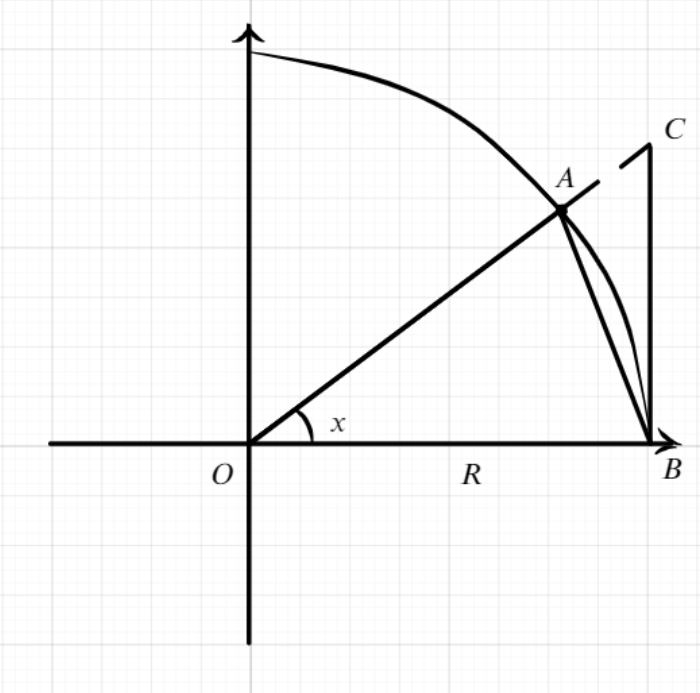
\includegraphics[scale=0.5]{images/img12.png}$$
\begin{center}
	пл. $\Delta ABO <$ пл. сектора $ABO<$ пл. $\Delta COB$;\\
	$\dfrac{1}{2}R^2 sin x < \dfrac{1}{2}R^2 x < \dfrac{1}{2}R^2 tg x$;\\
	$\sin x<x<\tg x\quad\Ra\quad\dfrac{1}{sinx}>\dfrac{1}{x}>\frac{1}{tgx}$.\\
\end{center}
Умножим на $\sin x$:
\begin{center}
	$1>\dfrac{\sin x}{x}>\cos x$.\\
\end{center}
Умножим на $-1$ и добавим $1$.
\begin{center}
	$0<1-\dfrac{\sin x}{x}<1-\cos x=2\sin^2\dfrac{x}{2}<2\sin\dfrac{x}{2}<x$.\\
\end{center}
Итак $0<1-\dfrac{\sin x}{x}<x\Ra$ по теореме о сжатой переменной, что $1-\dfrac{sinx}{x}\to0$ при $x\to+0$.\\
т.е. $\lim\limits_{x\to+0}\dfrac{\sinx}{x}=1$.\\
Если $x<0$, то $\lim\limits_{x\to-0}\dfrac{\sinx}{x}=\lim\limits{x\to-0}\dfrac{\sin(-x)}{(-x)}=\lim\limits_{y\to+0}\dfrac{siny}{y}=1$.\\\\
$$\lim\limits_{x\to0}\dfrac{\sinx}{x}=1.$$\\
\textbf{Замечание.} Из доказательства следует, что $\sinx\leqslant x$; $|\sinx|\leqslant|x|$.
\section{Замечательный степенно-показательный предел.}
$$\lim\limits_{x\to\infty}\Big(1+\dfrac{1}{x}\Big)^x=e.$$
\begin{Proof}
	Для доказательства используем критерий Гейне\\
	Для справедливости утверждения нужно показать, что $\forall(x_n)$, $x_n\to\infty$ $\Ra$ $\Big(1+\dfrac{1}{x_n}\Big)^{x_n}\to e$.
	\begin{enumerate}
		\item $x_n = n$, тогда $\Big(1+\dfrac{1}{n}\Big)^n\to e$. Этот результат нам уже известен из предыдущего.
		\item $x_n = k_n$, $(k_n)$ --- произвольная (не обязательно строго возрастающая последовательность натуральных чисел,  такая, что $k_n\to+\infty$.\\\\
		Так как $a_n = \Big(1+\dfrac{1}{n}\Big)^n \to e$ при $b \to +\infty$, то $$\forall \epsilon > 0,\ \exists\nu_\epsilon,\ \fa n \geqslant \nu_\epsilon \Ra |a_n - e | \leqslant \varepsilon.$$
		Поскольку $k_n \to \infty$, то 
		$$\fa M > 0,\ \exists \mu_M,\ \fa m \ge \mu_m\Ra k_m \ge M.$$
		Положим $M = \nu_\eps$. Тогда для $n \ge \mu_M$ выполняется $k_n \ge \nu_\eps$ и, следовательно, $|a_n - e|\le \eps$, что означает, что $a_{k_n} =\Big(1+\dfrac{1}{k_n}\Big)^{k_n} \to e $ при $n \to \infty$.
		\item Пусть $x_n \to \infty$. Любое $x_n$ можно заключить между двумя натуральными, то есть $\exists k_n$ такое, что $k_n \leq x_n < k_n+1$. Отсюда следует, что $$\dfrac{1}{k_n}\ge \dfrac{1}{x_n}\ge \dfrac{1}{k_n + 1}\Ra 1 + \dfrac{1}{k_n} \ge 1 + \dfrac{1}{x_n} \ge 1 + \dfrac{1}{k_n + 1}.$$
		Возводя в соответствующие степени, получим
		$$\Big(1 + \dfrac{1}{k_n}\Big)^{k_n} + \Big(1+ \dfrac{1}{x_n}\Big)^{x_n} + \Big(1+\dfrac{1}{k_n + 1}\Big)^{k_n + 1}.$$
		Тогда $$\Big(1 + \dfrac{1}{k_n} \Big)^{k_n} =\underbrace{\Big(\dfrac{1}{k_n + 1}\Big)^{k_n + 1}}_{\to e}\cdot\underbrace{ \dfrac{1}{\frac{1}{k_n + 1}}}_{\to 1}\rightarrow e,$$
		то есть $$\Big(\dfrac{1}{k_n + 1}\Big)^{k_n + 1} = \Big(1 + \dfrac{1}{k_n} \Big)^{k_n}\cdot \Big(1 + \dfrac{1}{k_n} \Big)\rightarrow e.$$
		Из теоремы о сжатой переменной $\Big(1+\dfrac{1}{x_n}\Big)^{x_n}\to e$, $n \to \infty$.
		\item Пусть $x_n \to \infty$. Обозначим $y_n ::= -x_n$. Имеем $$\Big(1+\dfrac{1}{x_n}\Big)^{x_n} = \Big(1-\dfrac{1}{y_n}\Big)^{-y_n} = \Big(\dfrac{y_n - 1}{y_n}\Big)^{-y_n} = \Big(\dfrac{y_n}{y_n - 1}\Big)^{y_n} = \Big(1 + \dfrac{1}{y_n - 1}\Big)^{y_n - 1}\cdot \Big(1 + \dfrac{1}{y_n - 1}\Big) \rightarrow e.$$
		Таким образом, $\Big(1+\dfrac{1}{x_n}\Big)^{x_n}\rightarrow e$ $\forall (x_n)\rightarrow \infty$. Поэтому на основании критерия Гейне $\Big(1+\dfrac{1}{x}\Big)^{x}\rightarrow e$ при $x \to \infty$.
	\end{enumerate}
\end{Proof}
\begin{corollary}
	Если $\alpha(x) \ne 0$ для всех $x$ из некоторой проколотой окретсности точки $x_0$ и $\alpha(x)\to 0$ при $x\to x_0$, то 
	$$\lim\limits_{x\to x_0}(1 + \alpha(x))^{\frac{1}{\alpha(x)}} = e.$$
	А в частности 
	$$\lim\limits_{x\to 0}(1 + x)^{\frac{1}{x}} = e.$$
\end{corollary}
\section{Асимптотическое поеведение функций.}
Начнем с примера. Пусть $\pi (x)$ --- количество простых чиел, не превосходящих данного действительного числа $x$. При каждом конкретном $x$ мы можем вычислить $\pi (x)$ простым перебором. У нас нет формулы для вычислений. Мы сразу не можем ответить и на вопрос, как ведет себя функция $\pi (x)$ при $x\to +\infty$, или, другими словами, каков асимптотический закон распределения простых чисел. От Евклида известно, что $\pi(x) \to +\infty$ при $x \to +\infty$, но доказать, что $\pi (x)$ растет примерно как $\dfrac{x}{\ln x}$ удалось только в прошлом веке русскому математику Чебышеву.\\\\
Когда нужно выяснить, как ведет себя функция в окрестности некоторой точки (или бесконечности), в которой, как правило, функция не определена, говорят, что интересуются асимптотикой или асимптотическим поведением этой функции в окрестности рассматриваемой точки.\\\\
Асимптотическое поведение функции обычно характеризуют с помощью другой, более частой, или более изученной функции, которая в окрестности исспледуемой точки с малой относительной погрешностью воспроизводит значение изучаемой функции.\\\\
Так, $\pi (x)$ при $x \to +\infty$ ведет себя как $\dfrac{x}{\ln x}$; функция $\dfrac{\sin x}{x}$ при $x \to 0$ ведет себя, как постоянная $1$; $\Big(1 + \dfrac{1}{x}\Big)^{x^2}$ ведет себя как $e^x$ при $x \to +\infty$; $x^2 + x + \sin \dfrac{1}{x}$ при $x \to +\infty$ ведет себя как $x^2$, а при $x \to 0$ как $\sin \dfrac{1}{x}$.\\\\
Перейдем теперь к точным определениям.
\section{Сравнение бесконечно малых функций.}
Пусть $f$ и $g$ заданы на проколотой окрестности $\dot{u}(a)$ точки $a$ и $\lim\limits_{a}f = 0$, $\lim\limits_{a}g = 0$, то есть $f$ и $g$ --- бмф.\\\\
$\bullet$ \textit{Будем говорить, что бмф $f$ является бмф \textbf{более высокого порядка} чем $g$ при $x \to a$ и $g$ является бмф \textbf{меньшего порядка} чем $f$, если $\lim\limits_{a}\dfrac{f}{g} = 0$. Запись: $f = o(g)$ при $x\to a$.}\\
\begin{example}
	$x ^ 2 = o (x)$, $x^3 = o(x)$, $\sin ^2 x = o(x)$, $x^3 = o(\sin x)$ при $x\to 0$.
\end{example}\\\\
$\bullet$ \textit{Функции $f$ и $g$ называем функциями \textbf{одного порядка малости} при $x \to a$, если $\lim\limits_{a}\dfrac{f}{g} = c$, $c \ne 0$, $c \ne \infty$.}\\\\
Иногда в этом случае пишут $f = O^*(g)$ при $x \to a$.\\\\
$\bullet$ \textit{Запись $f = O(g)$ при $x\to a$ означает, что $\exists M> 0 $, $\exists\dot{u}(a)$, что $\forall x \in \dot{u}(a)$ выполняется неравенство $|f(x)| \leqslant M\cdot|g(x)|$.}\\\\
\begin{theorem}
	Если $f = O^*(g)$, то $f = O(g)$ при $x\to a$.
\end{theorem}\begin{Proof}
	$f = O^*(g)\Rightarrow \exists c \in \Rm$, $c \ne 0$, $c \ne \infty$: $\lim\limits_{a}\dfrac{f}{g} = c$, то есть $$\forall \eps,\ \exists \delta(\eps) > 0,\ \forall x : 0 < |x - a| \leqslant \delta(\eps)\Rightarrow \Big|\dfrac{f}{g} - c\Big|\leq \eps \Longleftrightarrow c - \eps \leq \dfrac{f}{g} \leq c + \eps\Rightarrow$$
	$\dfrac{f}{g}$ ограничено. Тогда $\exists M : \Big|\dfrac{f}{g}\Big| \leq M \Rightarrow |f| \leq M \cdot |g|$ для $x \in ]a - \delta(\eps); a[$ $\cup$ $]a; a + \delta (\eps)[\Rightarrow f =~O(g).$
\end{Proof}\\\\
Отметим, что обратно, вообще говоря, неверно.\\
\begin{example}
	$x\sin \dfrac{1}{x} = O(x)$ при $x\to 0$, однако $x\sin \dfrac{1}{x} \ne O^*(x)$.
\end{example}\\\\
Запись $f = o(1)$ при $x\to a$ означает, что $f$ --- бмф при $x\to a$.\\\\
Запись $f = O(1)$ при $x\to a$ означает, что $f$ ограниченая  в некоторой окрестности точки $a$.\\\\
$\bullet$ \textit{$O, o$ --- \textbf{символы Ландау}.}\\\\
При использовании равенств с символами Ландау следует иметь ввиду, что эти равенства не являются равенствами в обычном смысле этого слова.\\
\begin{example}
	$f = o(x)$, $g = o(x)$ $\not \Rightarrow f = g$ $(x^2 = o(x)$, $x^3 = o(x))$.  
\end{example}\\\\
Для этих символов своя арифметика, так как символы $o$ и $O$ могут означать не только конкретные функции, но и классы функций. Более правильно было бы писать не $f= o(g)$, а $f \in o(g)$. Однако это затрудняет работу с этими символами.\\\\
\textbf{\textit{Основные правила $($при $x \to a)$:}}
\begin{enumerate}
	\item $o(g) + o(g) = o(g).$ (\textit{Суть} $f = o(g)$, $h o (g)\Rightarrow f + h = o(g)$.)
	\begin{Proof}
		Пусть $f = o(g)\Rightarrow \lim\limits_{a}\dfrac{f}{g} = 0$; $h = o(g)\Rightarrow\lim\limits_{a}\dfrac{h}{g}=  0$.
		Тогда $\lim\limits_{a} \dfrac{f + h}{g} = \lim\limits_{a}\dfrac{f}{g} + \lim\limits_{a}\dfrac{h}{g} = 0\Rightarrow f+h = o(g)$.
	\end{Proof}\\\\
	Аналогично доказываются следующие равенства
	\item $\alpha \cdot o(g) = o (\alpha g) = o (g)$, $\alpha \ne 0$.
	\item $f = o(g)\Rightarrow f = O(g)$.
	\item $o(f) + O(f) = O(f)$.
	\item $O(f) + O(f) =  O(f)$.
	\item $g \ne 0$, $\dfrac{o(f)}{g} = o\Big(\dfrac{g}{h}\Big);$ $\dfrac{o(f)}{g} = O\Big(\dfrac{g}{h}\Big)$.
	\item $O(\alpha f) = \alpha\cdot  O(f) = O(f)$.
	\item $o(f) \cdot O(f) = o(f)$.
\end{enumerate}
\section{Эквивалентные функции.}
$\bullet$ \textit{Бмф $f$ и $g$ называют \textbf{эквивалентными} при $x \rightarrow a$, если $\lim\limits_{a} \dfrac{f}{g} = 1$. Запись: $f \sim g$ при $x \rightarrow a$.}\\\\
Очевидно: $$f \sim g \Rightarrow g \sim f; \quad x \rightarrow a;$$
$$f \sim g,\ g \sim h \Rightarrow f \sim h; \quad x \rightarrow a.$$
\begin{example}
	$\sin{x} \sim x, \hspace{0.5 cm} 1 - \cos{x} \sim \dfrac{x^2}{2}, \hspace{0.5 cm} \tg{x} \sim x.$
\end{example}
\newtheorem*{keq}{Критерий эквивалентности функций}
\begin{keq} 
	$f \sim g$ при $x \rightarrow a \Longleftrightarrow f = g \oplus o(g)$ $(g = f \oplus o(f)).$ То есть бмф эквивалентны тогда и только тогда, когда разность между ними есть бмф более высокого порядка, чем каждая из них.
\end{keq}
\begin{Proof}
	\textbf{Необходимость}. Составим разность $h ::= f - g \Rightarrow \dfrac{h}{g} = \dfrac{f}{g} - 1 \Rightarrow \lim\limits_{a} \dfrac{h}{g} = 0 \Rightarrow h = o(g) \Rightarrow f - g = o(g) \Rightarrow f = g + o(g)$, $x \rightarrow a$.\\\\
	\textbf{Достаточность}. $f = g + o(g) \Rightarrow \dfrac{f}{g} = 1 + \dfrac{o(g)}{g} \Rightarrow \lim\dfrac{f}{g} = 1 \Rightarrow f \sim g$.
\end{Proof}
\begin{theorem}
	При вычислении пределов бмф можно заменять на эквивалентные в произведении.
\end{theorem}
\begin{Proof}
	Пусть $g \sim f, x \rightarrow a$. Tогда $\lim\limits_{a}g\cdot h = \lim\limits_{a}h \cdot \dfrac{g}{f}\cdot f = \lim\limits_{a}h\cdot f$.
\end{Proof}\\\\
Следует соблюдать осторожность при замене эквивалентным в сумме или разности.\\
\begin{example}
	$\lim\limits_{x \rightarrow 0} \dfrac{1 - \cos{(1 - \cos{x}})}{\sin^2{2x^2}} = \lim\limits_{x \rightarrow 0} \dfrac{(1 - \cos{x})^2}{8 x^4} = \dfrac{1}{32};$\\
	$\lim\limits_{x \rightarrow 0} \dfrac{\sin{x} - \tg{x}}{\sin{x^3}} = \dfrac{1}{2}.$\\\\
	\underline{Нельзя:} $\lim\limits_{x \rightarrow 0} \dfrac{x - x}{x^3} = 0$.
\end{example}
\section{Выделение главной части бмф.}
Пусть $f$ --- бмф при $x \rightarrow a$.\\\\
$\bullet$\textit{ Если $f = g + o(g)$, то $g$ называют \textbf{главной частью} бмф $f$ (то есть если $f \sim g$)}.\\\\
По бмф $f$ ее главная часть определяется, вообще говоря, неоднозначно.\\
\begin{example}
	$f = x + x^2 + x^3 + x^4 \Rightarrow f = x +o(x),\ f = x + x^2 + o(x)$ .
\end{example}\\\\
Чаще всего указывают вид главной части, либо вид главной части вытекает из той задачи, которую приходится решать.\\\\
Наиболее часто выделяют главную часть степенного вида $A(x - a)^k,\ A \neq 0,\ k > 0$.
$$f \sim A(x - a)^k$$
Если главная часть вида $A(x - a)^k$ существует, то она определяется единственным образом.
\section{Сравнение ббф.}
$f$ и $g$ --- ббф, $\lim\limits_{a}f = \infty,\ \lim\limits_{a}f = \infty$.\\\\
Если $ \lim\limits_{a}\dfrac{f}{g} = 0$, то $\begin{cases} f \text{ меньшего порядка, чем } g;\\
	g \text{ более высокого порядка, чем } f. \end{cases}$\\\\
$f = o(g): \vert f \vert \leqslant M\cdot \vert g \vert \Rightarrow f = O(g)\\
\dfrac{f}{g} \rightarrow 1 \Rightarrow f \sim g$\\\\
Выделение главной части.
$$x \rightarrow a - 0, a + 0, \infty, -\infty, +\infty.$$
\section{Непрерывность и ее геометрический смысл}
Пусть $f: X \rightarrow Y$, где $X$ --- множество, состояшее из одного или нескольких интервалов и $x_0$ --- внутренняя точка множества $X$, то есть
$$\exists U(x_0), \text{что } U(x_0) \subset Xю$$
$\bullet$ \textit{Функция $f$ называется \textbf{непрерывной в точке} $x_0$, если}
$$\lim\limits_{x \rightarrow x_0} f(x).$$
Непрерывность, как следует из определения, означает, что операция вычисления значения функции и перехода к пределу перестановочны, то есть
$$\exists \lim\limits_{x \rightarrow x_0} f(x) = f(x_0)$$
$$\lim\limits_{x \rightarrow x_0} f(x) = f(\lim\limits_{x \rightarrow x_0} x)$$
$\bullet$ \textit{\textbf{Непрерывность} функции $f$ \textbf{в точке} $x_0$ означает }
$$\forall \varepsilon > 0,\ \exists \delta_\varepsilon > 0,\ \forall x \in X,\ \vert x - x_0 \vert \leqslant \delta_\varepsilon\ \Rightarrow\ \vert f(x) - f(x_0) \vert \leqslant \varepsilon.$$
Здесь опущено требование по сравнению с пределом функции $0 < \vert x - x_0 \vert$, то есть мы допускаем случай $x = x_0$, более того, мы должны его рассматривать, так как в определении непрерывности участвует значение функции в точке $x_0$ , то есть $f(x_0)$. Заметим, что в точке  автоматически выполняется последнее неравенство, так как $f(x) - f(x_0)$ при $x = x_0$ равно нулю.\\\\
Вспомним определение предела функции в равносильной форме. Тогда\\\\
$\bullet$ \textit{Функция $f$ \textbf{непрерывна в точке} $x_0$, если}
$$\forall V(f(x)\ \exists U(x_0),\ f(U(x_0)) \subset V(f(x_0)).$$
Используя критерий Гейне, можно сказать и так:\\\\
$\bullet$\textit{ Функция $f$ \textbf{непрерывна в точке} $x_0$, если}
$$\forall (x_u),\ x_u \rightarrow x_0,\ x_u \in D(f)\ \Rightarrow \ f(x_u) \rightarrow f(x_0),\ u \rightarrow \infty.$$
Можно сказать и так:
$$x - x_0 =:: \Delta x,\ f(x) - f(x_0) = f(x_0 + \Delta x) - f(x_0) =:: \Delta f(x_0) = \Delta y.$$
$\bullet$ \textit{Функция $f$ \textbf{непрерывна в точке} $x_0$, если}
$$\forall \varepsilon > 0,\ \exists \delta_\varepsilon > 0,\ \forall x \in D(f), \ \vert \Delta x \vert \leqslant \delta _\varepsilon \ \Rightarrow \ \vert \Delta f(x_0) \vert \leqslant \varepsilon.$$
\subsection{Геометрический смысл непрерывности.}
Непрерывность в точке $x_0$ означает, что какую бы горизонтальную полоску ширины $2 \varepsilon$ ни взять, существует вертикальная полоска ширины $2 \delta_\varepsilon$ такая, что все точки графика, попадающие в вертикальную полоску, лежат и в горизонтальной, то есть попадают в прямоугольник.
$$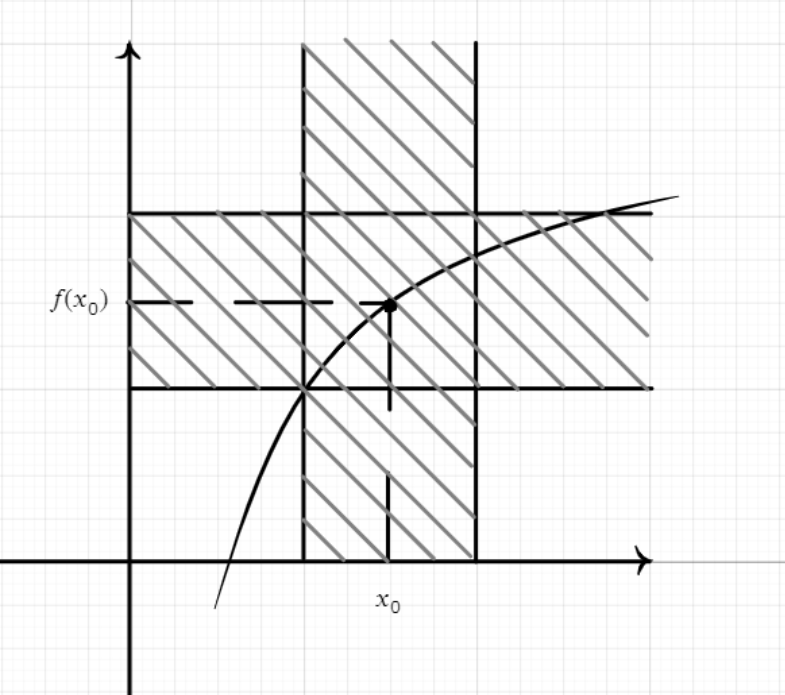
\includegraphics[scale=0.5]{images/img13.png}$$
Пусть теперь  $D(f) = [x_0; b[$, то есть $f$ задана в точке $x_0$ и справа от нее.\\\\
$\bullet$ \textit{Если существуют $\lim\limits_{x \rightarrow x_0}f(x) = f(x_0 + 0)$ и $f(x_0) = f(x_0 + 0)$, то функцию $f$ называют \textbf{непрерывной в точке} $x_0$ \textbf{справа}.}\\\\
Аналогично определяется и непрерывность слева.\\\\
По определению считаем $f$ непрерывной в изолированной точке.\\\\
$\bullet$ \textit{Функцию $f$ называем \textbf{непрерывной на множестве} $X$, если она непрерывна в каждой точке этого множества.}\\\\
Множество всех функций, непрерывных на множестве $X$ будем обозначать символом $\mathcal{C}(X)$.\\\\
Запись $f \in \mathcal{C}([a; b])$ обозначает, что $f$ непрерывна на отрезке $[a; b]$.
\section{Локальные свойства непрерывных функций.}
$\bullet$ \textit{\textbf{Локальными} называют такие свойства функции, которые определяются поведением функции в сколько угодно маленькой окрестности точки множества задания.}\\\\
Сами локальные свойства характеризуют поведение функции в каком-то предельном отношении, когда аргумент функции стремится к исследуемой точке. Например, непрерывность функции в некоторой точке множества задания, очевидно, есть локальное свойство функции.\\\\
\textbf{\textit{Локальные свойства непрерывных функций:}}
\begin{enumerate}
	\item \textit{Если $f$ непрерывна в точке $x_0$, то $f$ ограничена в некоторой окрестности $U(x_0)$.}
	\begin{Proof}
		Так как $f$ непрерывна в точке $x_0$, то $\exists \lim\limits_{x_0} f = f(x_0)$. А всякая функция, имеющая конечный предел в точке $x_0$, ограничена в окрестности этой точки.
	\end{Proof}
	\item \textit{Если $f$ и $g$ непрерывны в точке $x_0$, то в этой точке непрерывны и следующие функции:}
	$$\alpha f + \beta g \quad(\alpha, \beta \textit{ --- постоянные}); \quad f\cdot g;\quad \dfrac{f}{g} \quad (g \neq 0).$$
	\begin{Proof}
		Например, для $h = \dfrac{f}{g}$ выполняется $\lim\limits_{x \rightarrow x_0} h(x) = \lim\limits_{x \rightarrow x_0} \dfrac{f(x)}{g(x)} = \dfrac{\lim\limits_{x_0} f}{\lim\limits_{x_0} g} = \dfrac{f(x_0)}{g(x_0)} = h(x_0).$
	\end{Proof}
	\item \textit{Если $f$ непрерывна в точке $x_0$ и $f(x_0) \neq 0$, то существует такая окрестность точки $x_0$ для всех $x$, из которой $\sgn (f(x)) = \sgn (f(x_0)).$}
	\begin{Proof}
		$$\varepsilon := \dfrac{\vert f(x_0) \vert}{2},\ \exists \delta > 0,\ \forall x \in D(x), \vert x - x_0 \vert \leqslant \delta \Rightarrow \vert f(x) - f(x_0) \vert \leqslant \dfrac{\vert f(x_0) \vert}{2},$$ $$f(x_0) - \dfrac{\vert f(x_0) \vert}{2} \leqslant f(x) \leqslant f(x_0) + \dfrac{\vert f(x_0) \vert}{2}.$$
		\begin{enumerate}
			\item $f(x_0) > 0 \Rightarrow f(x) \geqslant f(x_0) - \dfrac{f(x_0)}{2} = \dfrac{f(x_0)}{2} > 0$
			\item $f(x_0) < 0 \Rightarrow f(x) \leqslant f(x_0) - \dfrac{f(x_0)}{2} = \dfrac{f(x_0)}{2} < 0$
		\end{enumerate}
		Итак, для $x \in [x_0 - \delta; x_0 + \delta] \Rightarrow \sgn(f(x)) = \sgn(f(x_0))$.
	\end{Proof}\\\\
	Это свойство называют еще \textbf{теоремой о стабилизации знака}.
	\item \textit{Для непрерывности функции $f(x)$ в точке $x_0$, являющейся внутренней для $D(f)$ необходимо и достаточно, чтобы $ \exists \, f(x_0-0), \, f(x_0+0) \,$ и при этом $f(x_0-0)=f(x_0)=f(x_0+0)$.}
	\begin{Proof}
		Непрерывность в точке $x_0$ означает, что $\lim\limits_{x \to x_0} f=f(x_0)$. А нам известно, что для существования предела функции необходимо и достаточно, чтобы существовали $f(x_0-0), \, f(x_0+0) \, $ и их совпадение.
	\end{Proof}\\\\
	Последним свойством чаще всего пользуются для исследования непрерывности функции, заданной различными формулами на разных промежутках.
\end{enumerate}
\section{Классификация точек разрыва}
$\bullet$ \textit{Пусть $x_0$ --- предельная точка множества $D(f)$ --- множества задания функции $f$. Точку $x_0$ называют \textbf{точкой разрыва} функции $f$, если $f$ не является непрерывной в этой точке.} \\\\
Как уже отмечалось, для непрерывности $f$ в точке $x_0$, необходимо и достаточно условия $f(x_0 - 0)=f(x_0)=f(x_0+0)$.
Поэтому, если функция разрывна в точке $x_0$, то нарушено одно из усиливающихся требований:
\begin{enumerate}
	\item пределы $f(x_0-0), f(x_0+0)$ существует;
	\item пределы $f(x_0-0), f(x_0+0)$ конечны;
	\item $f(x_0-0)=f(x_0+0)$;
	\item $f(x_0-0)= f(x_0+0) = f(x_0)$.
\end{enumerate}
В связи с этим\\\\
$\bullet$ \textit{Точка $x_0$ называется в случаях}
\begin{enumerate}
	\item $\nexists f(x_0-0) \vee \nexists f(x_0+0) \Rightarrow x_0$ \textit{\textbf{точкой неопределённости}};
	\item $f(x_0-0) \vee f(x_0+0)$  \textit{бесконечны $\Rightarrow x_0 $--- \textbf{точкой бесконечного скачка}};
	\item $f(x_0-0) \ne f(x_0+0) \Rightarrow x_0$ --- \textit{\textbf{точкой скачка}};
	\item $f(x_0-0) = f(x_0+0) \ne f(x_0) \Rightarrow x_0$ ---\textit{ \textbf{точкой устранимого разрыва}}.
\end{enumerate}
Разрыв $4$ можно устранить, доопределив или переопределив функцию в точке $x_0$.\\\\
$\bullet$\textit{ $1$ и $2$ --- точки разрыва \textbf{II-ого рода}; $3$ и $4$ --- точки разрыва \textbf{I-ого рода}}.\\
\begin{example}\begin{enumerate}
		\item 	$y = \sin{\dfrac{1}{x}}$, $x \ne 0$, $y(0)=1$;
		\item $y = \dfrac{1}{x}$, $y(0) = 1$;
		\item $y = 1(x)$;
		\item $y = 1(x)+1(-x)$.
	\end{enumerate}
\end{example}\\
$\bullet$ \textit{Функцию $f$ называют \textbf{кусочно-непрерывной} на $X$, если на любом конечном промежутке (или объединении конечного числа промежутков их $X$) из $X$
	функция $f$ имеет лишь конечное число точек разрыва, причём только первого рода.}\\\\
Каждую кусочно-непрерывную функцию можно представить в виде произведения непрерывной и кусочно-постоянной функций.
\section{Монотонные функции}
Пусть $f:D \rightarrow E$.
\begin{itemize}
	\item $f$ \textit{\textbf{строго возрастает}, если} $\forall x_1,x_2 \in D, x_1 < x_2     \Rightarrow f(x_1) < f(x_2)$;
	\item $f$ \textit{\textbf{возрастает}, если} $\forall x_1,x_2 \in D, x_1 < x_2 \Rightarrow f(x_1) \leqslant f(x_2)$;
	\item $f$ \textit{\textbf{строго убывает}, если} $\forall x_1,x_2 \in D, x_1 < x_2 \Rightarrow f(x_1) > f(x_2)$;
	\item $f$ \textit{\textbf{убывает}, если} $\forall x_1,x_2 \in D, x_1 < x_2 \Rightarrow f(x_1) \geqslant f(x_2)$.
\end{itemize}
\begin{lemma}
	Пусть $f: D \rightarrow E$ --- монотонная функция. Тогда во всякой внутренней точке $x_0 \in D$ оба односторонних предела $f(x_0-0)$ и $f(x_0+0)$ существуют и конечны, причём для возрастающей функции
	$$f(x_0-0) \leqslant f(x_0) \leqslant f(x_0+0)$$
	для убывающей
	$$f(x_0-0) \geqslant f(x_0) \geqslant f(x_0+0).$$
\end{lemma}
$\bullet$ \textit{Таким образом,\textbf{ точками разрыва} монотонной функции могут быть только точки разрыва I-ого рода, а именно, точки скачка.}\\
\begin{Proof}
	Доказательство приведём для возрастающей функции.
	Пусть $x_0$ --- внутренняя точка $D(f)$. Обозначим $X_{-} ::= \{x\ |\ x < x_0\}.$\\\\
	Тогда $f(x) \leqslant f(x_0)$, поскольку $f$ возрастает, множество $\{f(x)\ |\ x \in X\}$ не пусто, так как $x_0$ --- внутренняя точка, и множество ограничено сверху. Значит, у него существует верхняя граница. Обозначим её $A$, то есть $A::= \sup\{f(x)\ |x\ \in X_{-}\}$.\\
	$A \leqslant f(x_0)$, так как $f(x_0)$ --- мажоранта, а $A$ --- наименьшая из всех мажорант. Поскольку $A$ --- верхняя граница, то\\
	$$\forall \varepsilon >0,\ \exists x_1,\ x_1 < x_0 \Rightarrow f(x_1) > A - \varepsilon.$$
	Функция $f$ возрастает, поэтому $\forall x,\ x > x_1,\ x < x_0$
	$($то есть $x_1 < x < x_0) \Rightarrow f(x) \geqslant f(x_1) > A - \varepsilon$. 
	$x_0 - x_1 = ::\delta(\varepsilon)$\\
	Тогда $$A - \varepsilon \leqslant f(x) \leqslant A \leqslant A + \varepsilon.$$ Таким образом, имеем
	$$\forall \varepsilon > 0,\ \exists \delta_{\varepsilon} > 0\ (\delta_{\varepsilon} = x_0 - x_1),\ \forall x,\ 0 < x_0 - x \leqslant \delta(\varepsilon) \Rightarrow |f(x) - A| \leqslant \varepsilon.$$
	А это и означает, что $\exists f(x_0 - 0)$ и $f(x_0-0) = A$.\\
	А так как $A \leqslant f(x_0)$, то $f(x_0-0) \leqslant f(x_0)$.\\\\
	Аналогично доказывается, что $\exists f(x_0 +0)$ и $f(x_0) \leqslant f(x_0+0)$.
	(Рассматриваем $X_{+} = \{x | x > x_0\}, \inf{f(x) | x \in X_{+}}$.)\\\\
	Окончательно $f(x_0-0) \leqslant f (x_0) \leqslant f(x_0+0)$.
	Для убывающей функции доказательство приводится по этой же схеме.
\end{Proof}\\\\
\textbf{Замечание.} Отметим, что для возрастающей функции 
$$f(x_0-0) = \underset{x < x_0}{\sup}f(x),$$ $$f(x_0+0) = \underset{x > x_0}{\inf}f(x).$$
Попробуйте самостоятельно записать для убывающей функции.
\section{Критерий непрерывности монотонной функции.}
\newtheorem*{theorem_1}{Теорема}
\begin{theorem_1}
	Для того, чтобы монотонная функция $f: [a; b] \rightarrow E$ была непрерывна, необходимо и достаточно, чтобы множество значений этой функции было отрезком.\\
	$(f \in C([a; b]), f$ --- монотонная) $\Longleftrightarrow E(f) = f([a; b]) = [A; B]$ 
\end{theorem_1}
\begin{Proof}
	Проведём доказательство для возрастающей функции. Полагаем $f(a) = ::A, f(b) = ::B$. Если $A = B$, то отсюда следует с учётом монотонности, что $f$ --- постоянна и, значит, непрерывна.\\\\
	Пусть $A < B$.
	$A \leqslant f(x) \leqslant B, \forall x \in [a; b]$  из монотонности.
	$\forall x_0 \in ]a; b[ \Rightarrow f(x_0-0) \leqslant f(x_0) \leqslant f(x_0+0)$ по лемме.\\\\
	\textbf{Необходимость}.
	Пусть $f$ монотонно возрастает и непрерывна на $[a; b]$. Требуется доказать, что $E(f) = [A; B]$, то есть нужно показать, что какое бы число $C$, $A < C < B$ ни взять, найдётся $x_0 \in ]a; b[$, что $f(x_0) = C$.\\\\
	Возьмём $\forall C \in ]A; B[$. Обозначим $X_{-}:: = \{x\ |\ f(x) < C \}$.
	$$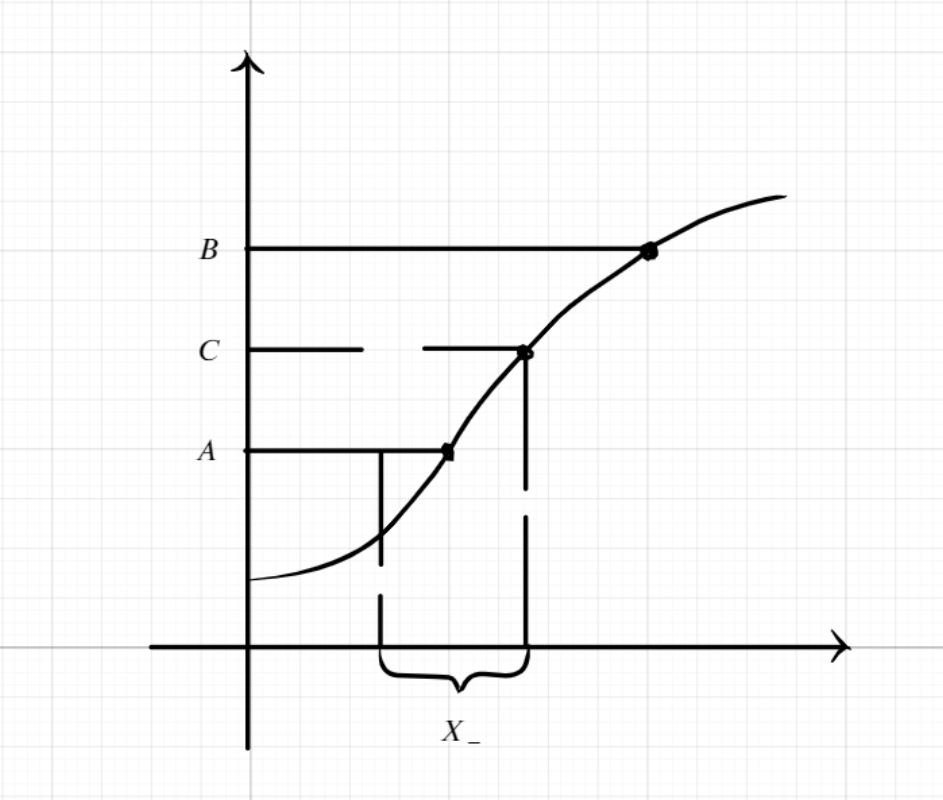
\includegraphics[scale=0.5]{images/img14.png}$$
	Множество $X_{-} \ne \varnothing$ (так как $a \in X_{-}$) и ограничено сверху (все $x \in [a; b]$). Поэтому у множества $X_{-}$ существует верхняя граница $x_0::= \sup{X_{-}}$.\\\\
	Ясно, что $f(x_0) \leqslant C$ (теорема о стабилизации знака).
	Для $x > x_0 \Rightarrow f(x) \geqslant C$,
	значит и $\inf{F(x)} \geqslant C$.
	Но $\inf{f(x)} = f(x_0 +0)$.
	Таким образом, $f(x_0 +0) \geqslant C$.
	Но $f$ непрерывна в точке $x_0$ и, поэтому, $f(x_0) = f(x_0+0)$.
	Таким образом приходим к неравенствам  $$C \geqslant f(x_0) = f(x_0+0) \geqslant C.$$
	Это возможно лишь в случае, если $f(x_0) = C$. Таким образом, для $\forall C \in ]A; B[$ нашлось $x_0 \in ]a; b[$, что $f(x_0) = C$. Это означает, что весь отрезок $[A; B]$ заполнен значениями функции $f$, то есть $E(f) = [A; B]$.\\\\
	\textbf{Достаточность}.
	Дано: $E(f) = [A; B] \quad f$ --- возрастает.
	Требуется доказать: $f \in C([a; b])$.
	Доказываем от противного.\\\\
	Пусть $f$ разрывна в некоторой точке $x_0 \in [a; b]$. Тогда (если $x_0$ --- внутренняя) нарушено условие $$f(x_0-0) = f(x_0) = f(x_0+0)$$ и, поскольку, на основании леммы
	$$f(x_0-0) \leqslant f(x_0) \leqslant f(x-0+0),$$ то либо $f(x_0-0) < f(x_0)$, либо $f(x_0) < f(x_0+0)$.\\\\
	Пусть, например, $f(x_0-0) < f(x_0)$.
	Выберем число $C$ так, чтобы $f(x_0-0) < C < f(x_0)$ (между двумя неравными числами всегда можно вставить третье).
	Ясно, что $C \in ]A; B[$.
	Тогда $$\forall x, x \geqslant x_0 \Rightarrow f(x) \geqslant f(x_0) > C,$$
	$$\forall x, x < x_0 \Rightarrow f(x) \leqslant \underset{x < x_0}{\sup}f(x) = f(x_0-0) < C.$$
	Оказалось, что ни в одной точке отрезка $[a; b]$ значение $C$ не принимается функцией $f$, что противоречит тому, что $E(f) = [A; B]$.\\\\ Аналогично рассматривается и случай $f(x_0) < f(x_0+0)$, то есть
	$$\exists C: f(x_0) < C < f(x_0+0);\ x \leqslant x_0 \Rightarrow f(x) \leqslant f(x_0) < C.$$
	$$x > x_0 \Rightarrow f(x) \geqslant \underset{x > x_0}{\inf}f(x) = f(x_0+0) > C$$
	и $C$ не является значением функции.\\\\ Полученное противоречие говорит о том, что допущение о разрывности $f$ в точке $x_0$ неверно, то есть функция $f$ обязана быть непрерывной на отрезке $[a; b]$.
\end{Proof}
\section{Непрерывность обратной функции}
Если $f: X \rightarrow Y$ и $f$ --- биекция, то как уже отмечалось во второй лекции, $\exists f^{-1}: Y \rightarrow X$.\\\\
Исследуем случай, когда $f$ строго монотонна и поставим вопрос: является ли она обратимой, то есть существеут ли для неё обратная функция $f^{-1}$?\\\\
Для этого достаточно, чтобы $f$ была биекцией, то есть, чтобы $f$ была инъективной и сюръективной, так как $f$  строго монотонна, например, для определённости, строго возрастающей, то из $x_1 > x_2 \Rightarrow f(x_1) > f(x_2)$, то есть $x_1 \ne x_2 \Rightarrow f(x_1) \ne f(x_2)$. Это значит, что $f$ инъективна. Для того, чтобы $f$  была и сюръективной, нужно потребовать, чтобы $Y = f(x) = E(f)$. Таким образом, приходим к следующей теореме.
\newtheorem*{theorem_11}{Теорема}
\begin{theorem_11}
	Строго монотонная функция $f: X \rightarrow Y$ является обратимой, то есть для неё существует обратная функция $f^{-1}: Y \rightarrow X$, если $f(x) = Y$. При этом обратная функция $f^{-1}$ будет строго монотонной в том же смысле, что и $f$.
\end{theorem_11}
\begin{Proof}
	Заключительное утверждение теоремы очевидно.\\\\
	Обозначим $y = f(x)$, $y_1 = f(x_1)$, $y_2 = f(x_2) \Rightarrow x_1 = f^{-1}(y_1)$, $x_2 = f^{-1}(y_2)$.\\\\
	Функция $f$ строго возрастает $\Rightarrow x_2 > x_1 \Rightarrow y_2 > y_1 \Rightarrow y_2 > y_1 \Rightarrow x_2 > x_1$, то есть $f^{-1}(y_2) > f^{-1}(y_1)$.
\end{Proof}
\newtheorem*{theorem_2}{Теорема о непрерывности обратной функции} 
\begin{theorem_2}
	Если $f$ чтрого монотонна и непрерывна на отрезке $[a; b]$, то она обладает обратной функцией, которая так же строго монотонная и непрерывна на отрезке с концами $[f(a); f(b)]$.
\end{theorem_2}
\begin{Proof}
	На основание предыдущей теоремы вытекает, что $f^{-1}$ существует и является чтрого монотонной функцией в том же смысле, что и $f$. Поэтому остаётся доказать только непрерывность $f^{-1}$.\\\\
	Пусть, для определённости, $f$ строго возрастает. На основании критерия непрерывности монотонной функции, её значения сплошь заполняют отрезок $[A; B] = [f(a); f(b)]$. Как мы уже отметили, $\exists f^{-1}$ и $f^{-1}$ строго возрастает на $[A; B]$, а так как $f^{-1}(y) = f^{-1}(f(x)) = x, \forall x \in [a; b]$, то множество значений обратной функции является отрезком $[a; b]$. По критерию непрерывности монотонной функции $f^{-1}$ непрерывна на $[f(a); f(b)]$.
\end{Proof}
\section{Непрерывность композиции}
Пусть $f: X_1 \rightarrow Y_1$, $g: X_2 \rightarrow Y_2$ и предположим, что $Y_2 \subset X_1$. Тогда можно рассматривать функцию $f_2: X_2 \rightarrow Y_1$, положив $h(x) = f(g(x))$.\\\\
$\bullet$ \textit{Такую функцию назовём \textbf{композицией (сложной функцией, суперпозицией)} функций $f$ и $g$. Причем $g$ --- \textbf{внутренняя функция}, $f$ --- \textbf{внешняя функция}. Обозначают композицию символом $f \circ g$. При этом важен порядок. Вообще говоря, $f \circ g \ne g \circ f$.}
\newtheorem*{theorem_4}{Теорема о непрерывности композиции}
\begin{theorem_4}
	Пусть функция $g: t \rightarrow g(t)$ непрерывна в точке $t_0 \in X_0$, а функция $f: x \rightarrow f(x)$, непрерывна в точке $x_0 = g(t_0) \in X_1$.
	Тогда функция $h = f \circ g$ непрерывна в точке $t_0$.
\end{theorem_4}
\begin{Proof}
	Пусть $f$ непрерывна в точке $x_0 \Rightarrow$
	\begin{center} $\forall \varepsilon > 0, \exists \delta_{\varepsilon} > 0, \forall x \in X_1, |x-x_0| \leqslant \delta_{\varepsilon} \Rightarrow |f(x) - f(x_0)| \leqslant \varepsilon.$\\ \end{center}
	Если $g$ непрерывна в точке $t_0 \Rightarrow$
	\begin{center} для $\delta_{\varepsilon}$ $\exists \Delta_{\varepsilon} > 0, \forall t \in X_2, |t-t_0| < \Delta_{\varepsilon} \Rightarrow |g(t)-g(t_0)| \leqslant \delta_{\varepsilon}$\\ \end{center}
	Рассмотрим для таких $t$ разность
	$$|h(t) - h(t_0)| = |f(g(t_0)) - f(g(t))| = |f(x) - f(x_0)| \leqslant \varepsilon.$$
	Итак, $$\forall \varepsilon >0,\ \exists \Delta_{\varepsilon} >0,\ \forall t,\ |t - t_0| \leqslant \Delta_{\varepsilon} \Rightarrow |h(t) - h(t_0)| \leqslant \varepsilon \Rightarrow$$ $h = f \circ g$ --- непрерывна в точке $t_0$.
\end{Proof}
\begin{corollary}
	Если $g \in C(X_2),\ f \in C(X_1) \Rightarrow f \circ g \in C(X_2)$.
\end{corollary}
\section{Непрерывность элементарных функций}
$\bullet$ \textit{Функции}
\begin{enumerate}
	\item $y = C$, \textit{то есть \textbf{постоянная}}; 
	\item $y = x^{\alpha}, \alpha \in \Rm$ --- \textit{\textbf{степенная}}; 
	\item $y = \sin{x}$, $y = e^{x}$  \textit{называются \textbf{простейшими элементарными функциями}.}
\end{enumerate}
$\bullet$\textit{ Всякая функция, составленная из простейших с использованием конечного числа следующих операций:}
\begin{enumerate}
	\item \textit{\textbf{арифметических}} $(+, -, \times, :)$,
	\item \textbf{\textit{композиции}},
	\item \textbf{\textit{обратной}},
\end{enumerate}
\textit{взятых в произвольном порядке, называется элементарной.}\\\\
\textit{\textbf{Примеры элементарных функций:}}
\begin{enumerate}
	\item постоянная $y = C$.
	\item идентичная $y = x$.
	\item степенная $y = x^{n}, n \in \N$.
	\item многочлен $P_{n}(x)$.
	\item рациональная $\frac{P_{n}(x)}{Q_{n}(x)}$.
	\item степенная $y = x^{\alpha}, \alpha \in \Rm$.
	\item экспонента $y = \exp^{x}$.
	\item показательная $y = a^{x} = \exp_{a}{x}$.
	\item логарифм $ y = \ln{x}, y = \log{a}{x}$.
	\item тригонометрические $\sin, \cos, \tan, \cot$.
	\item гиперболические $\sinh, \cosh, \tanh, \coth$.
	\item обратно тригонометрические $\arcsin, \arccos, \arctan, \dots$
	\item обратно гиперболические $arcsinh, arccosh, \dots$ 
\end{enumerate}
\textit{\textbf{Примеры неэлементарных функций}}
\begin{enumerate}
	\item $\sgn(x)$.
	\item $1(x)$.
	\item $|x|$.
\end{enumerate}
С помощью основных теорем о непрерывных функциях, можно показать, что все элементарные функции непрерывны там, где заданы (то есть непрерывны на множестве задания).\\\\
\begin{example}{ Обратные тригонометрические функции}
	$$y = \sh{x} = \frac{e^x - e^{-x}}{2};$$ $e^{x} = t$,
	$2y = t -\frac{1}{t} \Rightarrow t^2 - 2yt - 1 =0\\
	t_{1,2} = y \pm \sqrt{y^2+1}$, так как $t=e^x > 0 \forall x, t >0\\
	\Rightarrow t = y + \sqrt{y^2+1}$, то есть $e^x = y + \sqrt{y^2+1} \Rightarrow x = \ln{y + \sqrt{y^2+1}}$\\
	То есть $y = ln(x + \sqrt{y^2+1}$ --- функция обратная к $y = \sh{x}$. Обозначают $y = arsh(x)$\\
	Аналогично получаем:
	$y = arcch(x) = \ln{|x \pm \sqrt{x^2 -1}|}\\
	y = arth(x) = \frac{1}{2}ln{\frac{1+x}{1-x}}\\
	y = arcth(x) = \frac{1}{2}\ln{\frac{x+1}{x-1}}$
\end{example}
\section{Замечательные пределы}
\begin{enumerate}
	\item \textbf{Логарифмический предел}
	$$\underset{x \rightarrow 0}{\lim}{\dfrac{\ln{1+x}}{x}} = 1.$$
	\begin{Proof}
		$\lim{\dfrac{\ln{(1+x)}}{x}} = \lim{\ln({1+x}^{\frac{1}{x}})} = \ln{\underset{x \rightarrow 0}{\lim}({1+x}^{\frac{1}{x}})} = \ln{e} = 1$.
	\end{Proof}
	\begin{corollary}
		$$\underset{x \rightarrow 0}{\lim}{\dfrac{\log_{a}(1+x)}{x}} = \dfrac{1}{\ln{a}}.$$
	\end{corollary}
	\begin{Proof}
		$\underset{x \rightarrow 0}{\lim}{\dfrac{\log_{a}(1+x)}{x}} = \dfrac{\ln{(1+x)}}{\ln{a} \cdot x} \to \dfrac{1}{\ln{a}}.$
	\end{Proof}
	\item \textbf{Показательный предел}
	$$\underset{x \rightarrow 0}{\lim}{\dfrac{e^x-1}{x}} = 1$$
	\begin{Proof}
		$\dfrac{e^x-1}{x} = [ y = e^x-1, x= \ln{(1+y)}] = \dfrac{y}{\ln{(1+y)}} \xrightarrow[y \rightarrow 0]{} 1$
	\end{Proof}
	\begin{corollary}
		$$\underset{x \rightarrow 0}{\lim}{\dfrac{a^x-1}{x}} = \ln{a}.$$
	\end{corollary}
	\begin{Proof}
		$\underset{x \rightarrow 0}{\lim}{\dfrac{a^x-1}{x}} = \underset{x \rightarrow 0}{\lim}{\dfrac{e^{x \ln{a}}-1}{x}} = \ln{a}.$
	\end{Proof}
	\item \textbf{Степенной предел}
	$$\underset{x \rightarrow 0}{\lim}{\dfrac{(1+x)^{\mu}-1}{x}} = \mu.$$
	\begin{Proof}
		$\underset{x \rightarrow 0}{\lim}{\dfrac{(1+x)^{\mu}-1}{x}} = \lim{\dfrac{e^{\mu + \ln(1+x)}-1}{x}} \cdot \dfrac{\mu \ln{(1+x)}}{\mu \ln(1+x)} = \mu.$
	\end{Proof}
\end{enumerate}
\subsection{Линейная функция.}
$\bullet$ \textit{Функцию $y=k x$ называют \textbf{линейной} или линейным отображением.}\\\\
Иногда эту функцию обозначают $L$. $$L:\Rm\to\Rm,\qquad    L(x)=k x$$
$k$ --- коэффициент линейной функции.\\
Т.к. ${\Delta}L(x)=k \cdot {\Delta} x \to 0$ при ${\Delta}x \to 0$, то ${L}$ непрерывна в любой точке $\Rm$.\\\\
Всякая линейная функция определяется своим коэффициентом однозначно и, наоборот, всякое число $x\in\Rm$ определяет единственную линейную функцию.\\\\
Таким образом, между множеством линейных отображений и множеством действительных чисел существует взаимно-однозначное отображение или \textbf{луоморфизм}.\\\\
\textbf{\textit{Свойства линейной функции:}}
\begin{enumerate}
	\item \textit{$L(x_1+x_2)=L(x_1)+L(x_2),\ \forall x_1,x_2\in \Rm$.}
	\item \textit{$L(\alpha x)=\alpha L(x),\ \forall x\in\Rm,\ \forall \alpha\in\Rm.$}
\end{enumerate}
Иногда эти условия берут за определение линейной функции.
\section{Векторные и комплекснозначные функции.}
$\bullet$ \textit{Отображение $f:x\to\Rm^2,\ x\subset\Rm$, называют \textbf{векторной} функцией.}\\\\
Можно и $f:x\to\Rm^3$.\\\\
Другими словами \textbf{векторная функция} --- это отображение, которое каждому действительному числу состовляет вектор$$f:t\mapsto\vec r(t)=(x(t),\ y(t),\ z(t)).$$
Будем записывать $\vec r =\vec r(t)$
\begin{center}$\{$тройка чисел$\}\longleftrightarrow\{$точка $\Rm^3\}\longleftrightarrow\{$радиус-вектор точки$\}$
\end{center}
Задание вектор-функции равносильно заданию трех числовых (скалярных) функций.$$\vec r(t)=(x(t),\ y(t),\ z(t)).$$
$\bullet$ \textit{Вектор $\vec a$ называют \textbf{пределом векторной функции} $\vec r (t)$ при $t\to t_0$, если$$\forall \varepsilon>0,\:\exists \delta_\varepsilon>0,\: \forall t,\:0<|t-t_0|\leqslant \delta_\varepsilon \Rightarrow |\vec r(t)-\vec a|\leqslant \varepsilon $$}
Имеем:\[\lim_{t \to t_0} \vec r(t)=\vec a\Longleftrightarrow \lim_{t \to t_0}{|\vec r(t)-\vec a|}=0.\]
\textbf{Теорема.}
\textit{Если $\vec r(t)=x(t)\vec i +y(t)\vec j + z(t)\vec k$, то}  \[\lim_{t \to t_0} \vec r(t)=\vec a=a_1 \vec i+a_2 \vec j +a_3 \vec k \Longleftrightarrow \lim_{t \to t_0}x(t)=a_1,\: \lim_{t \to t_0}y(t)=a_2,\:\lim_{t \to t_0}z(t)=a_3.\]
$\bullet$ \textit{Векторная функция $\vec r(t)$ называется \textbf{непрерывной} в точке $t_0$, если} \[\lim_{t \to t_0} \vec \tau(t)=\vec\tau(t_0).\]
\textbf{Теорема.}
\textit{Для того, чтобы $\vec\tau(t)$ была непрерывной в точке $t_0$, необходимо и достаточно, чтобы в $t_0$ были непрерывны $x(t), y(t), z(t)$.}\\\\\
Аналогично вводится и понятие комплексозначной функции $$f:t\mapsto x(t)+i\cdot y(t)=::z(t).$$ $z(t)\underset{t\to t_0}\to C=A+i B$, если $|z(t)-C|\to 0$ при $t\to t_0$
$$z(t)\to C\Longleftrightarrow x(t)\to A,\ y(t)\to B,\ t\to t_0.$$
$z(t)$ непрерывна в $t_0$, если \[\lim_{t \to t_0}z(t)=z(t_0),\]
\begin{center}
	$(z(t)$ непрерывна в $t_0) \Longleftrightarrow(x(t), y(t)$ непрерывны в $t_0).$
\end{center}